\section{Euler-Gerade und Feuerbach-Kreis}
%
%
%
\subsubsection{Definition:}
$a,b,c$ sei ein Dreieck
\begin{enumerate}
	\item Seitenhalbierende: Verbindung von $\vec{a}$ mit $\frac{1}{2}(\vec{b}+\vec{c})$
	\item Mittelsenkrechte: Senkrechte auf $b-a$ durch $\frac{b-a}{2}$
	\item Höhe: durch $a$ ist das Lot von $a$ auf $c-b$
\end{enumerate}
%
%
%
\subsubsection{Satz:}
\begin{enumerate}
	\item Die Seitenhalbierenden schneiden sich in einem Punkt$s$: "`Schwerpunkt"'.
	\item Die Mittelsenkrechten schneiden sich in einem Punkt $m$: "`Schwerpunkt"'.
	\item Die Höhen schneiden sich in einem Punkt$h$: "`Höhenschnittpunkt"'.
\end{enumerate}
%
%
%
\subsubsection{Beweis:}
\begin{enumerate}
	\item $\vec{c}+\mathbb{R}(\frac{a+b}{2}-c)\mathop{=}\limits^{\textrm{Parameter 
	}\frac{2}{3}}\frac{a+b+c}{3}$\\
	Symmetrie $\Rightarrow$ auf allen Seitenhalbierenden.
	\item $2<a-b,x>=<a-b,a+b>=\Vert a\Vert^{2}-\Vert b\Vert^{2}$\\
	$2<b-c,x>=<b-c,b+c>=\Vert b \Vert^{2}-\Vert c \Vert^{2}$\\
	$2<c-a,x>=<c-a,c+a>=\Vert c \Vert^{2}-\Vert a\Vert^{2}$\\
	Addition liefert $0=0$
\end{enumerate}
$\Rightarrow$ Jede der Gleichungen ist Konsequenz der anderen beiden
%
%
%
\subsubsection{Satz (von Euler):}
$\vec{h}=\vec{s}+2(\vec{s}-\vec{m})$ insbesondere liegen $s,h,m$ auf einer Geraden
%
%
%
\subsubsection{Beweis:}
z.z. $\vec{h}=3\vec{s}-2\vec{m}=\vec{a}+\vec{b}+\vec{c}-2\vec{m}$
genauer: $\vec{a}+\vec{b}+\vec{c}-2m$ liegt auf jeder Höhe\\
Höhe durch $c: <a-b,x>=<a-b,c>$\\
$<a-b,a+b+c-2\vec{m}>=\mathop{\underbrace{<a-b,a+b>-<a-b,2\vec{m}>}}\limits_{=0}+<a-b,c>$
%
%
%
\subsubsection{Definition (von Feuerbach):}
Der Feuerbachkreis des Dreiecks $abc$ mit $s,h,m$ ist der Kreis durch die Seitenmitten. Sei $f$ sein Mittelpunkt.\\
%
%Grafik einfügen
%
\subsubsection{Satz:}
\begin{enumerate}
	\item $\vec{f}=\frac{\vec{h}+\vec{m}}{2}$ d.h. $f$ liegt auf der Euler-Geraden in der 
	Mitte zwischen $h$ und $m$.
	\item Radius d.Feuerbachkreises ist die Hälfte des Umkreisradius. 
	\item $\frac{h+a}{2} , \, \frac{b+h}{2}, \, \frac{h+c}{2}$ liegen auf dem Feuerbachkreis
	\item Fußpunkt der Höhen auch
\end{enumerate}
%
%
%
\subsubsection{Beweis:}
Verschiebe so, dass $s=\vec{0}$ also $a+b+c=0$ 
\begin{enumerate}
	\item $K$ ist Umkreis des 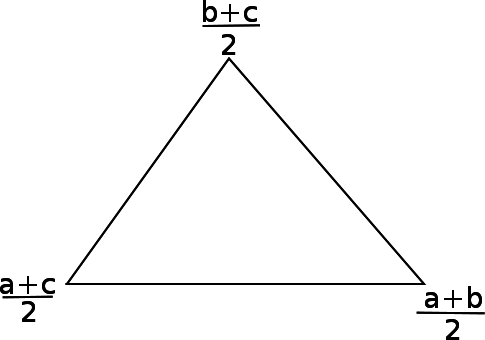
\includegraphics[width=0.2\textwidth]
	{mainmatter/chapter1/pics/dreieck1.png} durch die Seitenmitten $\Rightarrow f$ liegt 
	auf dessen Mittelsenkrechte, erfüllt daher \\ 
	$<\frac{a+c}{2}-\frac{b+c}{2},f>$\\
	$=<\frac{a+c}{2}-\frac{b+c}{2}, \frac{a+b+2c}{2}>$\\
	$= <a-b,f> -\frac{1}{4}\mathop{\underbrace{<a-b,a+b>}}\limits_{2<a-b,m>}$\\
	$=<a-b,-\frac{m}{2}$\\
	Genauso $<b-c,f>=<b-c,-\frac{m}{2}>,..., \text{d.h. }2f+m=\vec{0}$ tut's. f liegt auf 
	allen 3 Höhen durch $-\frac{m}{2} \Rightarrow f = -\frac{m}{2}$\\
	$\frac{1}{2}(h+m)\mathop{=}\limits^{\text{Euler}}\frac{1}{2}(-2m+m)=-\frac{1}{2}
	(-2f)=f$
	\item $r_{\text{K}}=\Vert f-\frac{a+b}{2}\Vert\mathop{=}\limits^{s=0}\Vert f+\frac{c}
	{2}\Vert = \Vert c-m \Vert = \frac{1}{2} \quad r_{\text{Umkreis}}$
	\item $\Vert \frac{h+a}{2}-f \Vert \mathop{=}\limits^{\text{Euler}}_{h=-2m (1.))}\Vert 
	-m+\frac{a}{2}+\frac{m}{2}\Vert = \frac{1}{2} \Vert m-a \Vert  
	\mathop{=}\limits^{2.)}r_{\text{K}}$
	\item Projeziere senkrecht auf die Seite $ab$. Dann geht 
	\begin{itemize}
		\item $h$ auf den Höhenfußpunkt $hc$
		\item m auf $\frac{a+b}{2}$
		\item und $f$ auf die Mitte dazwischen (nach 2.) 
	\end{itemize}
	$\Rightarrow$ Das Dreieck 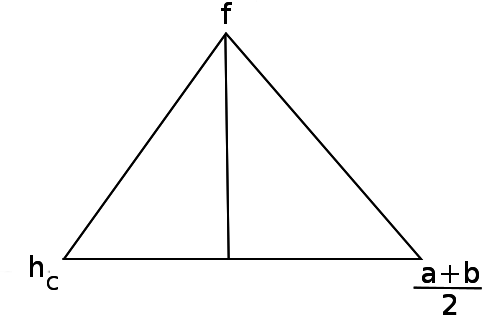
\includegraphics[width=0.2\textwidth]
	{mainmatter/chapter1/pics/dreieck2.png} ist gleichschenklig $\Vert hc-f \Vert = \Vert 
	\frac{a+n}{2} -f \Vert$ (Pythagoras)
	\begin{figure} [H]
	\centering
	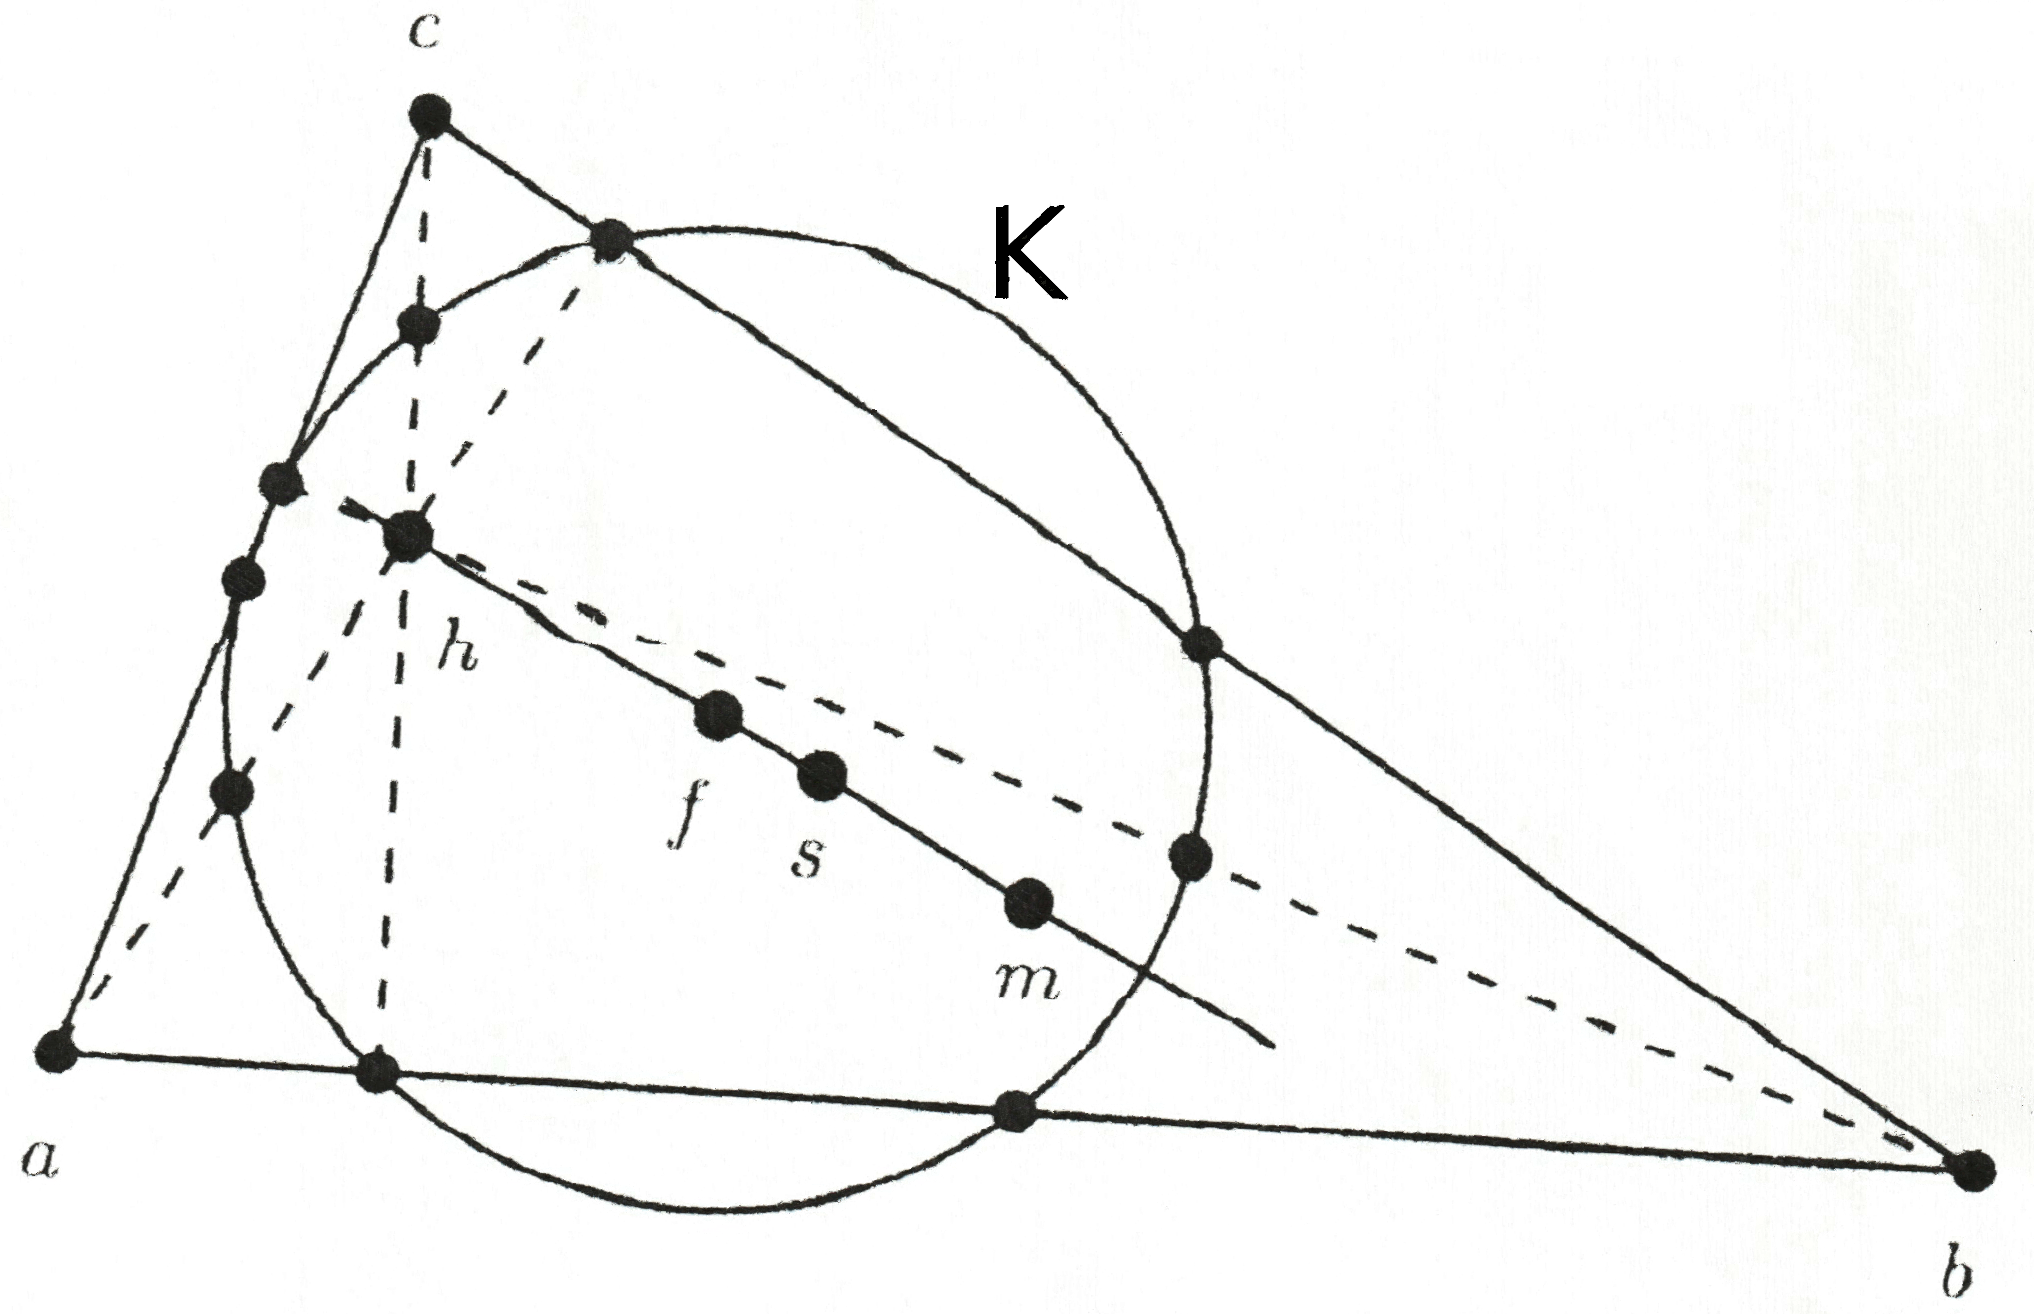
\includegraphics[width=0.45\textwidth]
	{mainmatter/chapter1/pics/feuerbachkreis.png}
	\caption{Der Feuerbachkreis}
	\end{figure}
\end{enumerate}
Projeziere $\mathcal{E}$ auf die Gerade $ab$. \\
Dann liegt das Bild von $f$ in der Mitte zum Seitenmittelpunkt und Fußpunkt der Höhe\\
$\Rightarrow \Vert f-\frac{a+b}{2}\Vert = r_{\text{F-Kreis}}=\Vert f-h_{c} \Vert$\\
$\Rightarrow h_{c}$ liegt auf dem F-Kreis\\
\qquad\\
\subsubsection{Korollar:}
$3s=m+2f$ DENN: $2f \mathop{=}\limits^{\text{F.}}h+m \mathop{=}\limits^{\text{E.}}3s-m \qquad \checkmark$